\documentclass[10pt,a4paper]{report}

\usepackage[utf8]{inputenc}
\usepackage[french]{babel}
%\usepackage{lmodern}%pour un meilleur rendu des polices
\usepackage{verbatim}%du texte non interprt
\usepackage{amsmath,amssymb}%maths
\usepackage{graphicx}%images
\usepackage{xspace}
\usepackage{color}%Couleurs
\usepackage{appendix}%annexe
\usepackage[a4paper, top= 2.5 cm, bottom = 2.5 cm, left = 2 cm, right = 1.5 cm] {geometry}
\usepackage{listings}
\usepackage[final]{pdfpages} 
\lstset{
  morekeywords={abort,abs,accept,access,all,and,array,at,begin,body,
      case,constant,declare,delay,delta,digits,do,else,elsif,end,entry,
      exception,exit,for,function,generic,goto,if,in,is,limited,loop,
      mod,new,not,null,of,or,others,out,package,pragma,private,
      procedure,raise,range,record,rem,renames,return,reverse,select,
      separate,subtype,task,terminate,then,type,use,when,while,with,
      xor,abstract,aliased,protected,requeue,tagged,until},
  sensitive=f,
  morecomment=[l]--,
  morestring=[d]",
  showstringspaces=false,
  basicstyle=\small\ttfamily,
  keywordstyle=\bf\small,
  commentstyle=\itshape,
  stringstyle=\sf,
  extendedchars=true,
  columns=[c]fixed
}


%\usepackage{lastpage}%nombre de pages
%En tte et pied de page<
\usepackage{fancyhdr}
\pagestyle{fancy}
\lhead{\sectionmark} 
\chead{}
\rhead{}
\lfoot{Projet BD 2012-2013}
\cfoot{\textbf{Romaric,Valmon,Thibault,Romain}}
\rfoot{\thepage\ }
\renewcommand{\headrulewidth}{0pt}  
\renewcommand{\footrulewidth}{0.4pt}
%Page de garde
\makeatletter
\def\thickhrulefill{\leavevmode \leaders \hrule height 1pt\hfill \kern \z@}
\def\maketitle{%
  \thispagestyle{empty}%
  \begin{center}
  \begin{flushleft}
  \normalfont\LARGE \par
	  \end{flushleft}
	\vskip 4.5cm
	  \leavevmode
	  \normalfont
	  \thickhrulefill\par
	  \vskip 0.2cm
	  {\huge\@title\par}%
	  \vskip 0.1cm
  \thickhrulefill\par
	  \vskip 1cm
	  {\Large \@date\par}%
  \vskip 12cm
  {\Large \@author\par}%
  \end{center}%
	  \clearpage
}



\title{Documentation de conception\\
{\em Projet de Base de Données}}
\author{Romarik JODIN\\ Valmon LEYMARIE\\ Romain KOENIG\\ RIHET Thibault}
\date{Vendredi 17 Mai 2013}
\begin{document}
\maketitle
\newpage
\tableofcontents
\newpage


\chapter*{Présentation du Projet}
\paragraph{}Lors de ce projet, nous nous proposons de réaliser une application de gestion d'un tournoi d'echec. Nous nous appliquerons lors de celui-ci à mettre en oeuvre les connaissances que nous avons acquise en cours d'ACVL, de gestion de base de données et de programation orientée objet pour analyser le sujet, concevoir la base de données et implémenter l'application en Java. 
\mbox{}\hspace{0.4cm}Notre application devra permettre à un organisateur de gérer les inscriptions et les phases du tournoi, à un observateur de regarder une rencontre en direct ou en différrer et à un joueur de jouer une partie d'echec.
\chapter{Analyse}
\paragraph{}Pour cette première partie d'analyse du sujet, nous avons décidé de rester tous ensemble afin de discuter de notre compréhension du sujet et de poser nos questions communes aux clients. Suite à cette étape, nous avons scindé le groupe en deux sous-groupes: Romaric et Valmon se sont chargés de réaliser l'analyse dynamique, tandis ce que Thibault et Romain ont étudié l'analyse statique.\\
\mbox{}\hspace{0.4cm}Nottons que malgré cette répartition, nos deux groupes n'ont jamais arrêté de communiquer afin de rester cohérent tout au long de ce projet.
\section{Analyse dynamique}
\subsection{Diagramme des cas d'utilistions}
\paragraph{}Dans un premier temps, nous avons identifié les acteurs (joueur, organisateur et spectateur) et les différents cas d'utilisation:
\begin{center}
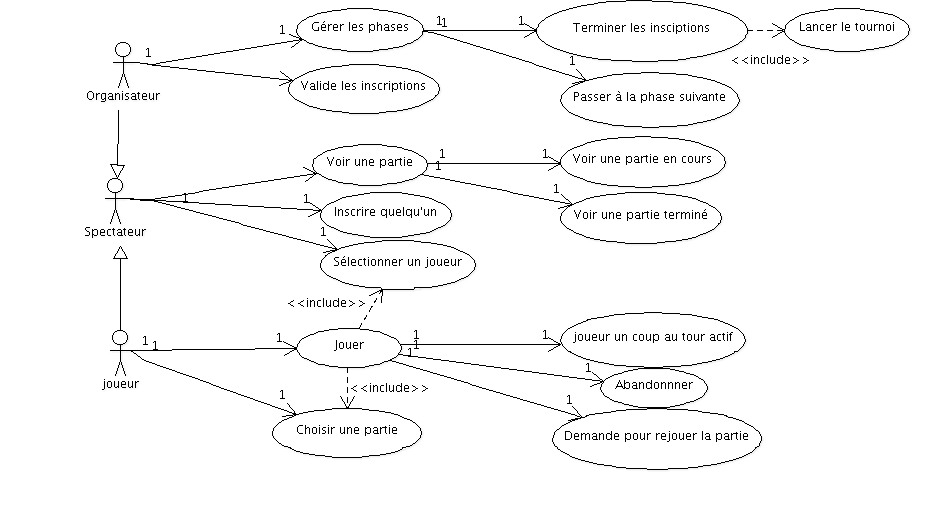
\includegraphics[width=18cm]{Diag_d_util.png}
\end{center}
\mbox{}\hspace{0.4cm}Nous avons estimé qu'un utilisateur était forcément un \textit{spectateur} avant de se rendre dans le menu \textit{organisateur} ou \textit{joueur}. Comme expliqué dans le sujet, un \textit{organisateur} peut soit valider une inscription, soit passer à la phase suivante, un \textit{spectateur} peut seulement regarder des rencontres en cours ou terminées, s'identifier parmis la liste des joueurs, ou se rendre dans le menu \textit{organisateur}, et enfin, un joueur peut sélectionner une partie pour la continuer si elle est en cours, et la commencer si elle ne l'est pas encore.

\subsection{Diagramme de séquence}
\paragraph{}Une fois les différents cas d'utilisations identifiés, nous nous sommes questionnés sur le fonctionnement de l'application. Ce raisonement nous a amené à établir plusieurs diagrammes de séquences qui illustrent différents déroulements possibles: 

\paragraph{Diagramme de séquence d'inscription} Pour ce diagramme de séquence, nous supposons que l'utilisateur n'est pas loggés et est donc un spectateur. Celui-ci envoie une demande, et compléte le formulaire adéquat. Une fois rempli, les informations du spectateur sont insérés dans la base de données dans la table \textit{DEMANDE\_INSCRIPTION}. Ensuite, un organisateur peut consulter la liste des demandeur d'inscription en consultant la base de données, et valider une inscription, ce qui aura pour effet de créer un nouveau joueur dans la table \textit{JOUEUR} et d'effacer le joueur de la liste des demandeurs d'inscription.
\begin{center}
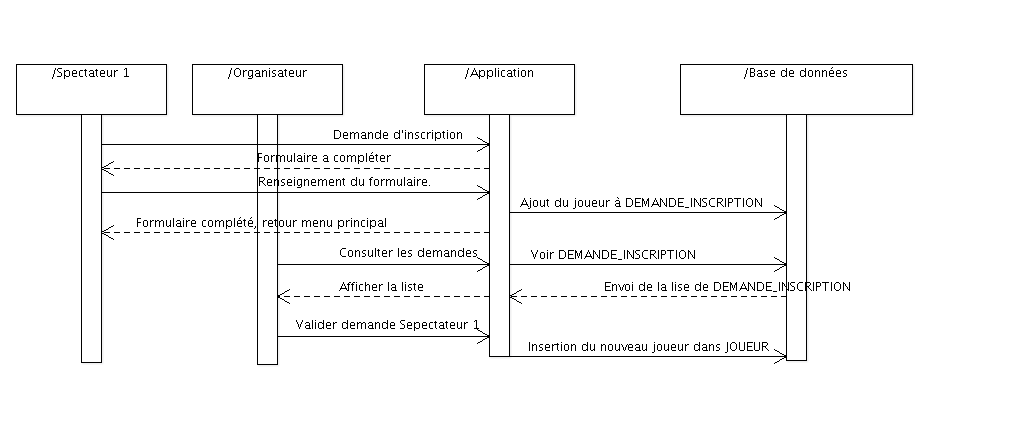
\includegraphics[width=18cm]{DiagSeqInscr.png}
\end{center}

\paragraph{Diagramme de séquence pour cloturer les inscriptions}Pour clôturer les inscriptions, on admettra que l'utilisateur est dans le menu organisateur de la phase d'inscription. Il demande la clôture des inscriptions, l'application interroge la base de données pour savoir si la table \textit{JOUEUR} contient au moins 8 tuples. Si c'est le cas, comme dans notre scénario, l'application crée toutes les rencontres dans la base de données et initialise les échiquiers de chaque rencontre. Enfin, l'application passe à la phase de jeu et affiche à l'utilisateur le menu principal de la phase de jeu. 
\begin{center}
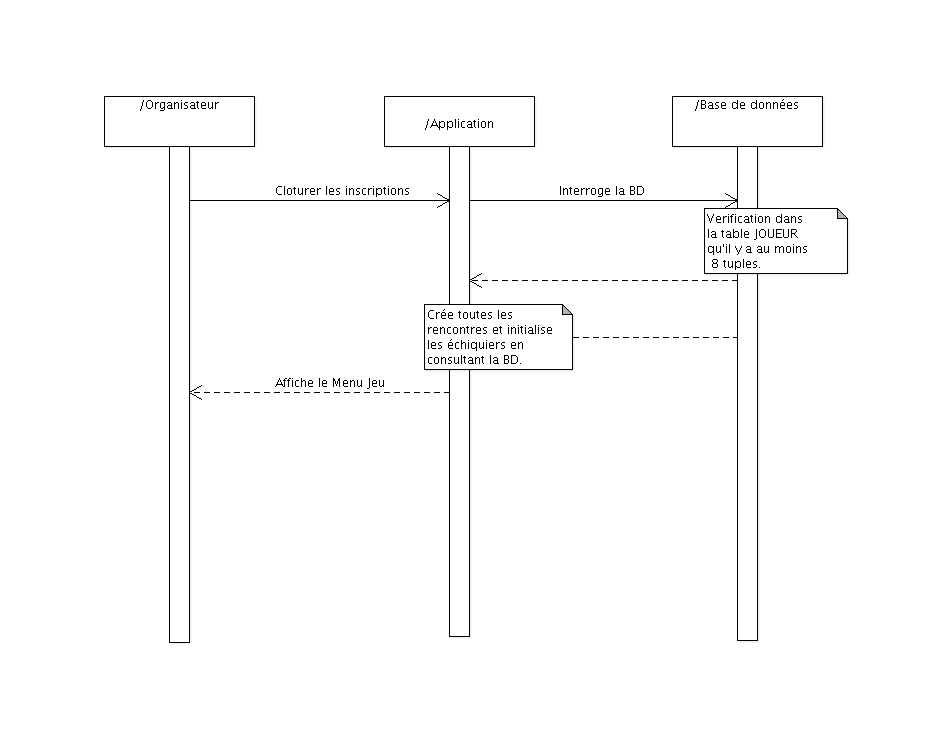
\includegraphics[width=18cm]{DiagSeqCloture.png}
\end{center}

\paragraph{Diagramme de séquence pour jouer un coup}Pour jouer un coup, on admettra qu'un joueur est identifié, à selectionné une partie est que c'est à son tour de jouer. Avant de jouer, l'application vérifie que le joueur qui a la main qu'il n'est pas en échec, nous supposerons que c'est le cas ici. Ensuite, le joueur peut jouer un coup. L'application vérifie alors que le coup est valide (c'est à dire que la pièce sélectionnée lui appartient,qu'il n'y a pas de pièce sur le chemin du déplacement, que la case d'arrivée ne soit pas occupée par une pièce qui lui appartient aussi..etc). Ensuite, l'application envoi le déplacement à la base de donnée, qui renvoi une erreur en cas de déplacement invalide. 
\begin{center}
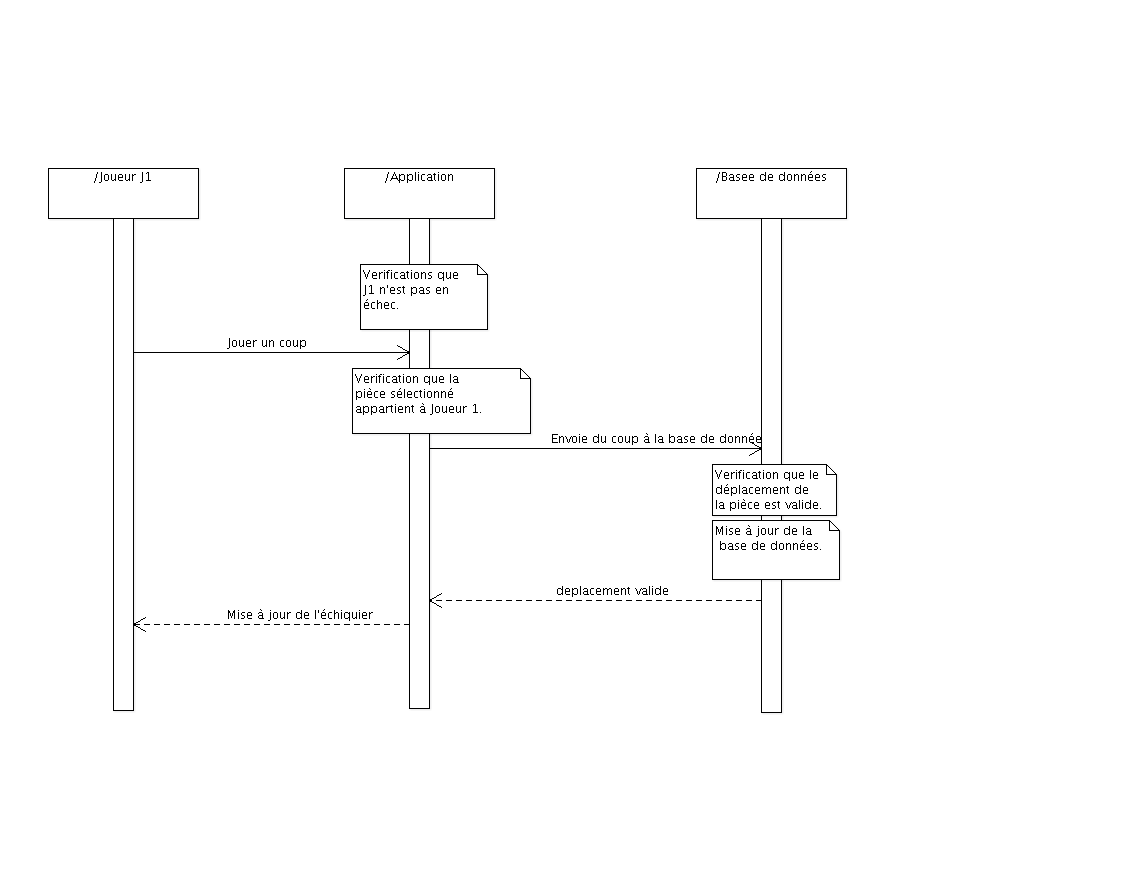
\includegraphics[width=18cm]{DiagSeqJouerCoup.png}
\end{center}


\paragraph{Diagramme de séquence pour le déroulement d'une partie entre plusieurs joueurs}}Nous avons ensuite illustré le déroulement du jeu lorsque plusieurs utilisateurs interagissent avec l'application. Le joueur J1 sélectionne une partie contre J2. Le systéme reçoit la requête du joueur et va chercher dans la base de données la position actuelle des pièces pour récupérer la position des pièces et afficher l'échiquier. Le systéme informe le joueur J1 qui a lancé la partie que ce n'est pas à son tour de jouer et qu'il doit patienter ou sélectionner une autre partie. Lorsque le joueur J2 lance la rencontre contre le joueur J1, l'application de la même façon va chercher dans la base de données la position des pièces et affiche l'échiquier. L'application informe ensuite J2 des actions disponibles: Jouer un coup, demander à rejouer la partie, abandonner la partie et retour au menu principal. Le joueur J2 joue alors son coup, et l'application interagit en conséquence avec la base de données (non détaillé ici car explicité dans le diagramme de séquence jouer un coup). Enfin l'application, affiche le nouvel échiquier, et informe le joueur J2 que ce n'est pas à son tour de jouer.
\begin{center}
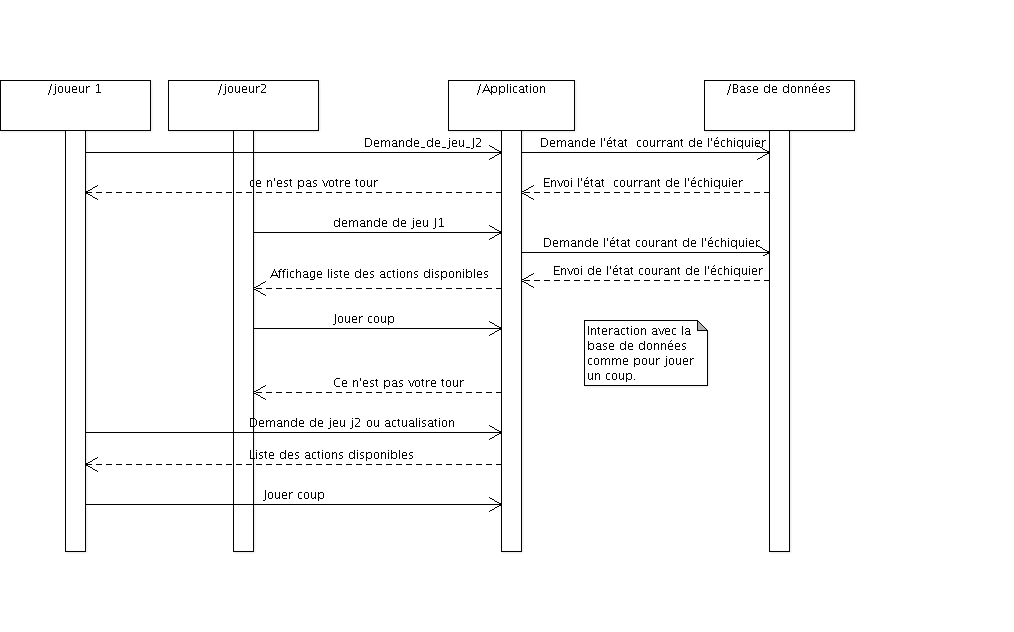
\includegraphics[width=18cm]{DiagSeqPlusieurJoueur.png}
\end{center}

\paragraph{Diagramme de séquence pour regarder une partie}Pour regarder une partie, nous admettrons que la phase courrante est une phase de jeu. L'utilisateur a directement accés au menu pour regarder une rencontre à partir du menu principal, comme il n'est pas loggé, cela fait de lui un \textit{spectateur}. Le spectateur choisit de regarder une rencontre depuis le début, l'application va donc chercher dans la base de données la liste de tous les matchs. Le spectateur selectionne une phase puis une rencontre, l'application consulte la base de données pour afficher l'échiquier de la phase saisie, de la rencontre saisie et du tour 0. L'utilisateur peut alors demander le coup suivant, dans quel cas, de la même façon, l'application va chercher dans la base de données pour la même phase, et la même partie le coup suivant. Si celui-ci a déjà été joué, on affiche l'échiquier pour le coup suivant, et si le coup suivant n'a pas encore été joué, l'application en informe le spectateur et affiche le même echiquier. 
\begin{center}
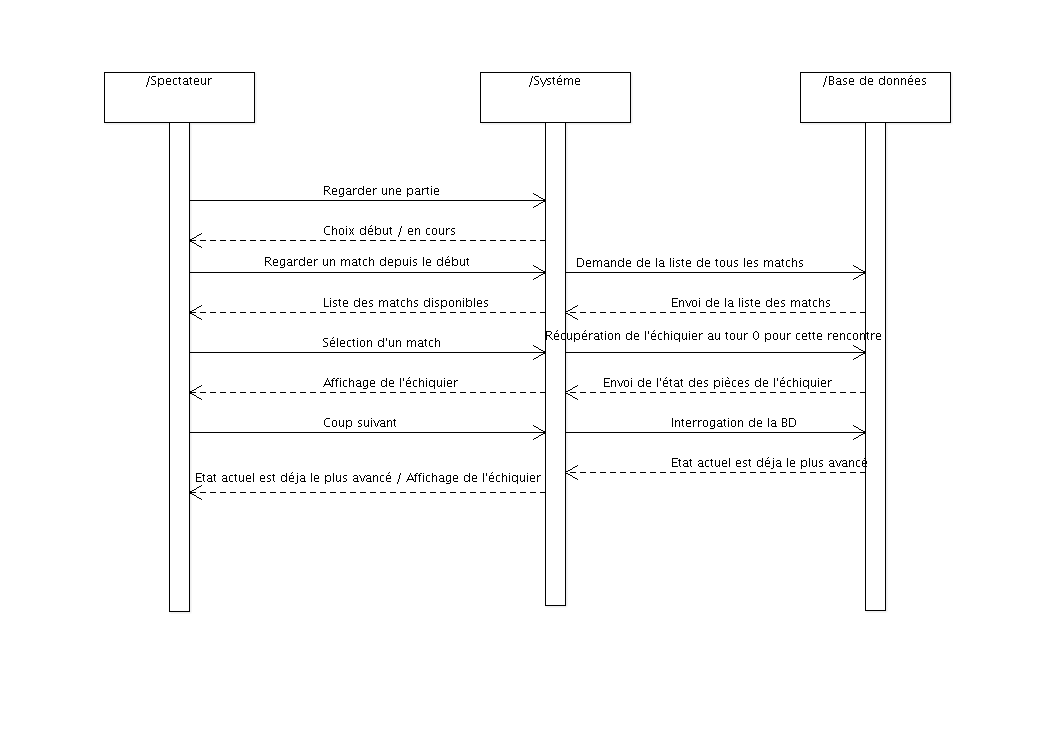
\includegraphics[width=18cm]{DiagSeqRegarderPartie.png}
\end{center}

\paragraph{Diagramme de séquence pour rejouer une partie}Pour ce scénario, on admettra être dans la phase de jeu. À n'importe quel moment, J1, qui joue contre J2 demande à rejouer la partie. L'application informe alors la base de données de cette demande du joueur J1. La base de données change la valeur de \textit{RESET\_REQUEST} pour la partie considérée. Lorsque le joueur J2 lance la partie avec J1, l'application l'informe que le joueur adverse a voulu rejouer la partie et laisse le choix à J2 de rejouer ou de continuer la partie en cours. Dans notre cas, J2 accepte de rejouer la partie, dans ce cas, l'application demande à la base de données de supprimer tous les tours joués et de remettre les pièces à leur position initiales. Le joueur qui joue le premier coup est le même que clui qui avait commencé la partie annulée.
\begin{center}
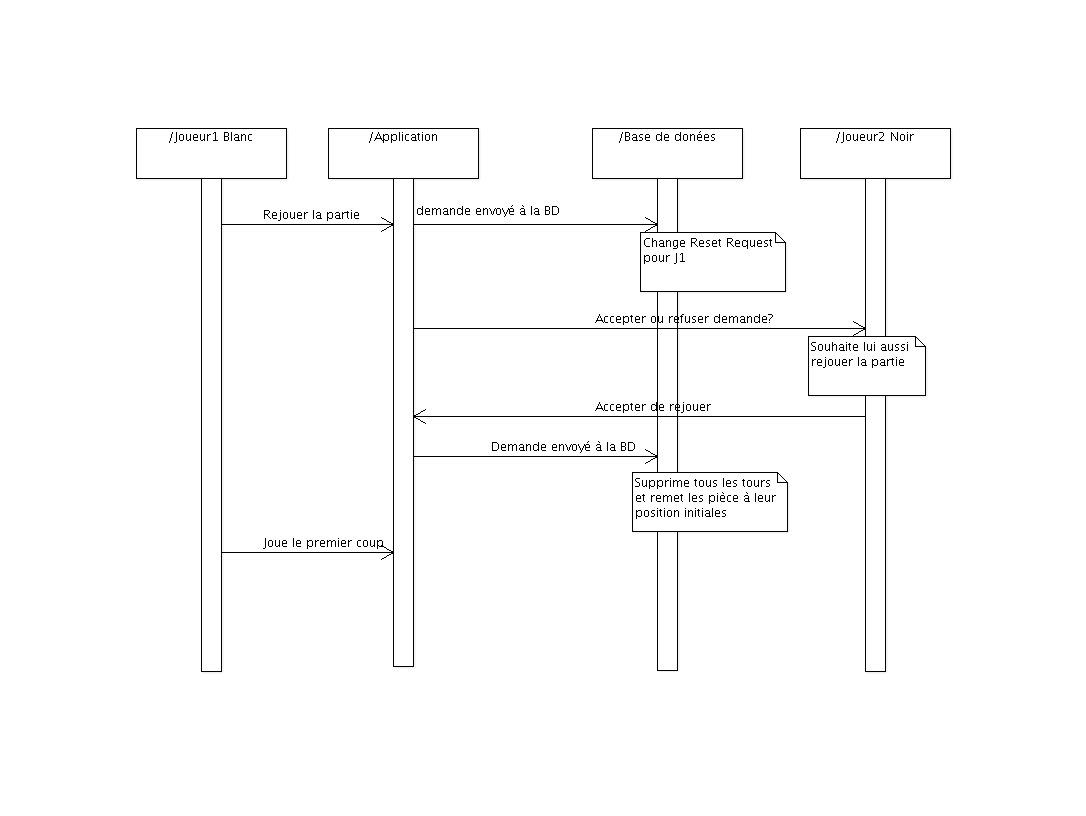
\includegraphics[width=18cm]{DiagSeqRejouerPartie.png}
\end{center}


\paragraph{Diagramme de séquence pour un échec}En cas d'échec, on admet que la partie est avancée et que le joueur J1 a choisit de jouer contre J2 qui vient de le mettre en échec. Dans ce cas, l'application informe J1 qu'il est en situation d'échec. J1 joue un coup, l'application vérifie entre autre que J1 n'est plus en échec, il envoie le coup à la base de données qui vérifie que le déplacement est valide. J2 joue à son tour et quand J1 lance de nouveau la partie contre J2, l'application vérifie si celui-ci est en situation d'échec, dans ce cas, il consulte les déplacements possibles des pièces dans la base de données lors de l'algorithme de calcul pour savoir s'il y a échec et mat. On admet ici que notre appication a trouvé une solution dans quel cas, il informe le joueur qu'il est en situation d'échec et lui propose la liste des actions disponibles.
\begin{center}
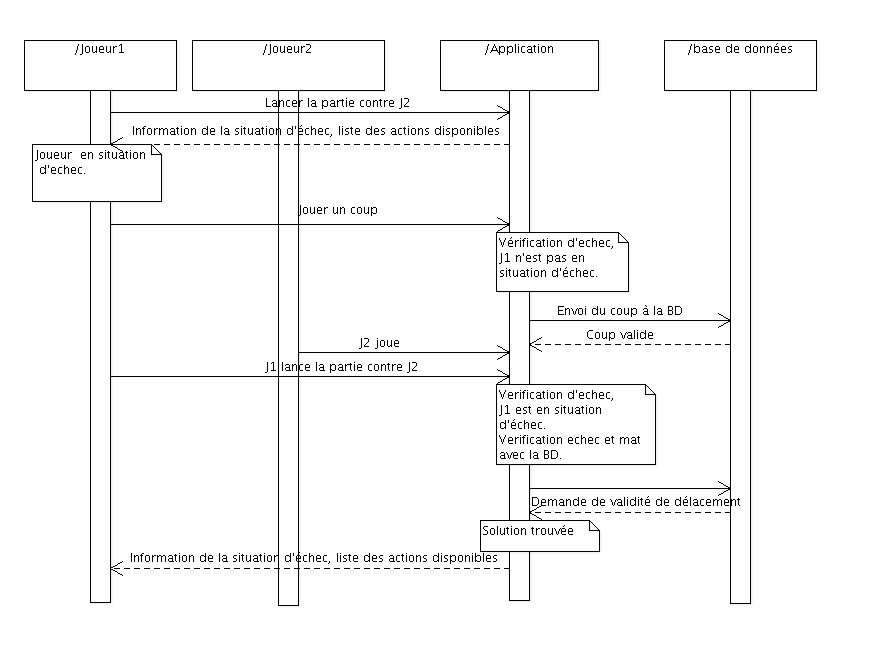
\includegraphics[width=18cm]{DiagSeqEchec.png}
\end{center}






\subsection{Diagramme d'état transition}
\paragraph{}Après avoir identifié les grandes phases du fonctionnement de notre application (inscription et jeu), nous nous sommes lancés dans la réalisation d'un diagramme d'états transition pour chacune d'entre elle:

\paragraph{Diagramme d'état transition pour la phase d'inscription}
\begin{center}
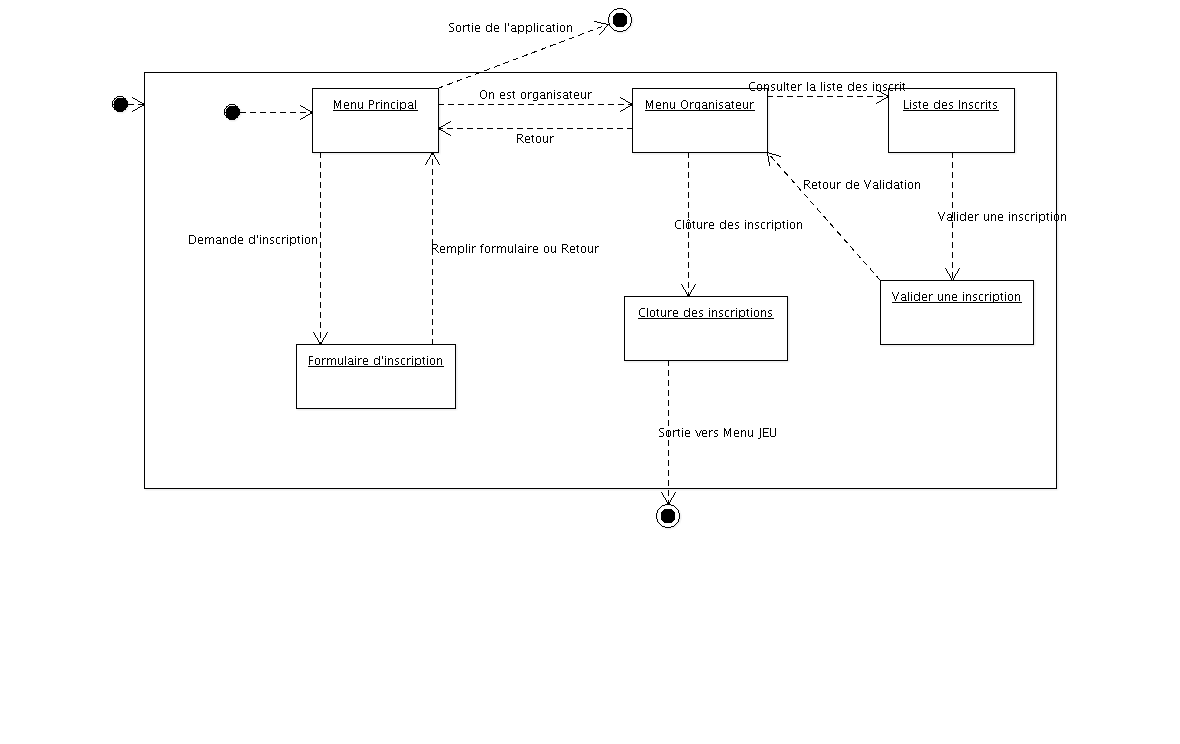
\includegraphics[width=17cm]{Etat_transi_Inscr.png}
\end{center}

\paragraph{Diagramme d'état transition pour la phase de Jeu}
\begin{center}
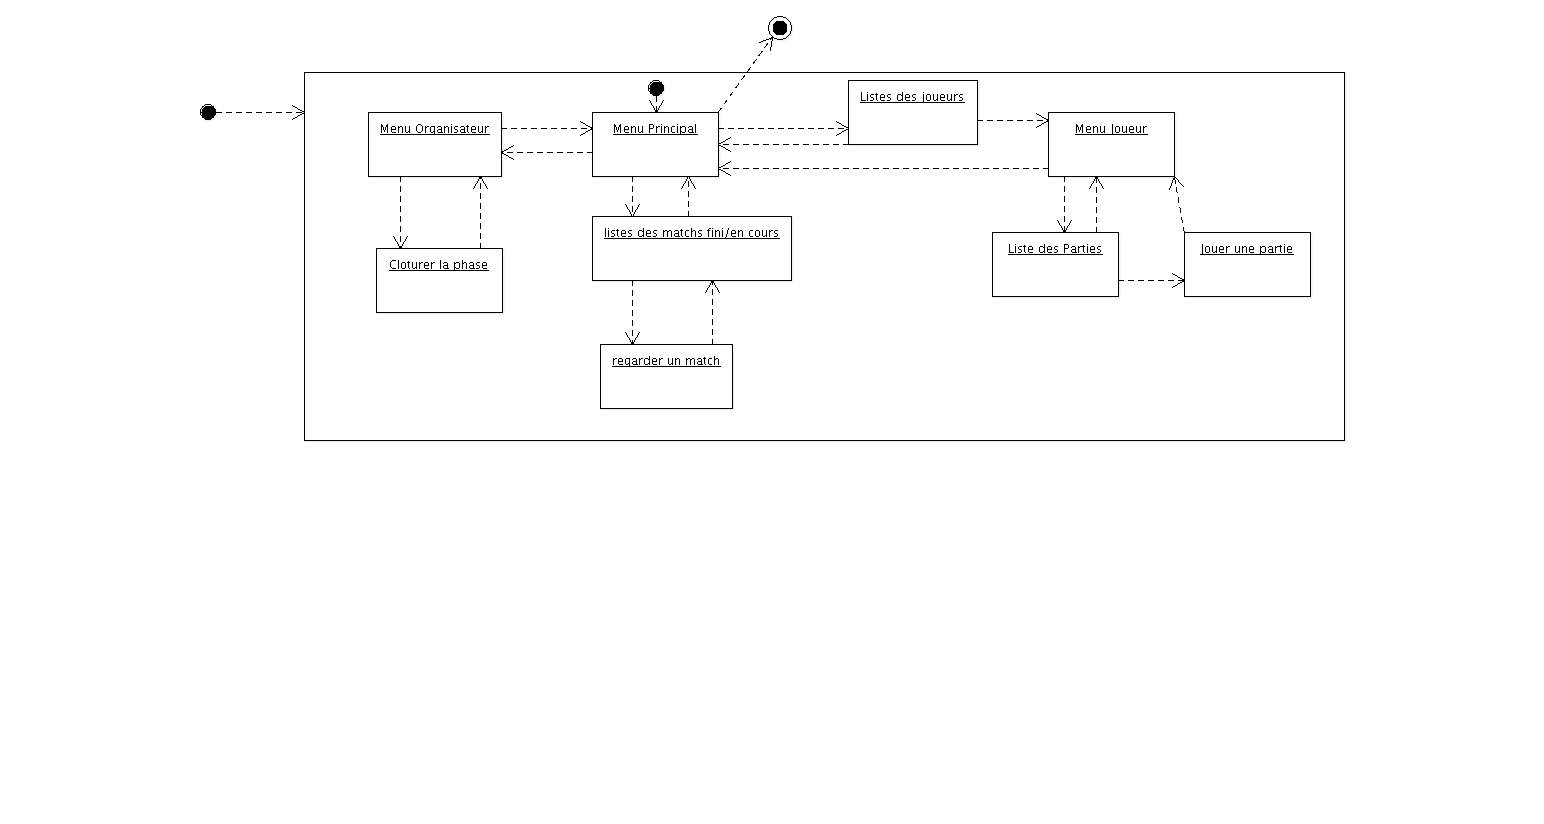
\includegraphics[width=17cm]{Etat_transi_Jeu.png}
\end{center}




\section{Analyse statique}
\paragraph{}

La première étape de la conception d'une base de donnée est d'extraire du texte les dépendances fonctionnelles et les contraintes qui doivent régir 
les données.
Cette analyse se base sur la compréhension du cahier des charges. De cette analyse, nous avons tiré le tableau suivant:
\begin{center}
\begin{array}{||p{5.1cm}||p{4.2cm}||p{3.8cm}||p{3cm}||}
\hline\hline
\textbf{Dependances fonctionnelles} & \textbf{Contraintes de valeur} & \textbf{Contraintes de multiplicite} & \textbf{Autre}\\
\hline\hline
idJ $\rightarrow$  Nom, Prenom, Adresse, Date & & & \\
\hline\hline
phase, idPartie $\rightarrow$ idJ1, idJ2, gagnant & gagnant $\in$ \{idJ1, idJ2, Undefined\} & Une rencontre a 2 joueurs et un gagnant & \\
\hline\hline
idJ , idPartie, idPhase $\rightarrow$ couleur & & & Dans une rencontre les 2 joueurs ne peuvent pas partager la même couleur \\
\hline\hline
idPhase, idPartie, idTour $\rightarrow$ idPiece & & A chaque tour on bouge une pièce & \\
\hline\hline
idPiece $\rightarrow$ couleur, x, y, preX, preY & 0 $\leq$ X $\leq$ 7 & & \\
& 0 $\leq$ Y $\leq$ 7 & & \\
& 0 $\leq$ preX $\leq$ 7 & &\\
& 0 $\leq$ preY $\leq$ 7 & &\\
& couleur $\in$  { noir, blanc } & & \\
& Déplacement valide: f(X,Y,preX,preY)=TRUE & & \\
\hline\hline
& & & On a besoin de connaître la phase de jeu courante\\
\hline\hline
& & & Les demandes d'inscription devront être validées par l'organisateur \\
\hline\hline
\end{array}
\end{center}


\chapter{Conception et implantation de la base de données}
\paragraph{}

\section{Conception de la base de données}
\subsection{Elaboration du schéma conceptuel}
\paragraph{}
On peut obtenir à partir de ce tableau le schéma entité/association de notre base de données. \\
\begin{center}
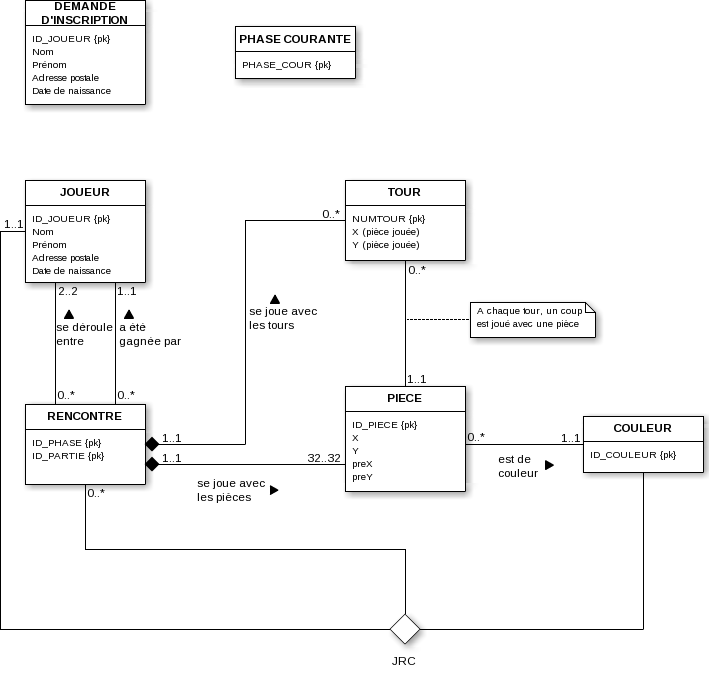
\includegraphics[width=12cm]{DiagEntiteAsso.png}
\end{center}
\mbox{}\hspace{0.4cm}Certaines tables ne sont pas reliés aux autres, en effet pour certains besoin de l'application nous avons du garder en donnée persistante certaines variable, comme la phase courante. Une simple table suffit à implémenter une telle variable et n'importe quelle application peut s'y référer.\\

\subsection{Conception de la base de données}
\paragraph{}
La base de données a été réalisée en SQL. Une traduction des relations et des contraintes a été effectuée en SQL pour obtenir les tables
contenues dans notre base de données. La création de ces tables est contenue dans le fichier \lstinline!create_table.sql!.
Ce fichier permet aussi de réinitialiser la base de donnée, en effet elle supprime toutes les tables de la base de donnée et les crées de nouveau, 
vide.

\section{Validation de la base de données}
\paragraph{}
La cohérence des données doit être validée dans une base de données. Pour cela plusieurs tests ont été menés, certains visant à valider le bon
fonctionnement de la base de données et d'autres visant à la rendre incohérente avec le cahier des charges.

\subsection{Tests en boite noire}
Une base de tests basée uniquement sur le cahier des charges a été effectuée. Cette série de tests vise à vérifier le bon fonctionnement de la base de 
données quant au cahier des charges. 
Ces tests correspondent donc à différentes utilisations possibles de la base de données et correspondent à des requêtes probables.
On trouvera notamment le fichier \lstinline!base.sql! qui initialise une rencontre entre deux joueurs. Ce script valide donc l'ensemble de la base de données
en ce qui concerne l'initialisation d'une rencontre. Il sert aussi de base pour mener d'autre tests.\\
D'autre part, un scripts pour inscrire des joueurs a été effectué: \lstinline!inscr.sql!. Ce script inscrit 8 joueurs dans la base de données.\\
Le script \lstinline!tour_jeu.sql! simule l'utilisation de la base de données pour effectuer différents coups dans une partie.

\subsection{Tests en boite blanche}
Une base de tests basée sur l'implémentation de la base de données a été effectuée. Cette série de tests valide des points spécifiques de l'implémentation
de la base de données.\\
Ces tests simulent des utilisations correctes ou non de la base de données en cherchant à valider les contraintes de la base de données.
Les tests invalides se situent dans le dossier \lstinline!invalide!. Dans le script \lstinline!id_joueur!, on cherche à inscrire deux fois le
même joueur. Dans le dossier \lstinline!Rencontre!, on cherche à créer une rencontre invalide (joueur qui joue contre lui même, incohérence
de couleurs, plus de deux joueurs dans une partie).\\
D'autre part il nous a fallu valider les contraintes sur le déplacement des pièces.
Pour ce faire dans le dossier "dossier", nous avons écrit plusieurs scripts pour automatiser les tests et réaliser un grand nombre de déplacements 
possible. Le premier script est \lstinline!gene_test_nomPiece.sh!. Ce script permet de générer tout les déplements possible d'une pièce à partir 
de sa position initial ( qu'on peut configurer dans \lstinline!base.sql! par exemple ).
Puis on lance le script \lstinline!generation_result.sh! qui va exécuter tout les tests précédemment créés, en se connectant automatiquement à 
la base de donnée et en enregistrant les résultats dans un fichier du même nom que le test et avec l'extention .lst.
Un dernier sript, du nom de \lstinline!compare.sh! permet de comparer les résultats générés avec une autre chaîne comme un résultat attentu,
ce qui permet ensuite de trouver automatiquement les fichiers qui fonctionne ou non, qui peuvent poser problème etc...
Ceci est fait pour chaque pièce de l'échiquier.

\subsection{Analyse des accès à la base de données}
\paragraph{}
La connection à la base de données depuis l'application se fait à
l'aide de l'interface proposée par JDBC. Les requêtes suivantes sont
des exemples de requêtes contenues dans le code Java pour accéder à la
base de données (en utilisant l'interface de JDBC). Certaines de ces
requêtes sont critiques dans le sens où elles nécessitent d'être
isolées. Plusieurs accès concurrent à la base de données risquent de
corrompre cette dernière et de fausser les données. Par défaut, le
mode d'isolation de \lstinline!SQL*PLUS! est \lstinline!READ
COMMITED!. Cela permet d'être sûr que la donnée n'est pas altérée
pendant la lecture. Le niveau d'isolation \lstinline!SERIALIZABLE! est
nécessaire lorsqu'on va modifier les données. Le détail des
requêtes à isoler est expliqué par la suite.

\paragraph{Fichier ProduitListeInscrit.java}
% du fichier PoduitListeinscrit
Accès à la BD pour rechercher les demandes d'inscriptions :
\begin{verbatim}
SELECT * FROM DEMANDE_INSCRIPTION
\end{verbatim}
\\
Modification de la BD pour ajouter un inscrit :
\begin{verbatim}
SELECT MAX(ID_JOUEUR) AS ID_JOUEUR FROM DEMANDE_INSCRIPTION GROUP BY ID_JOUEUR UNION ALL 
	SELECT MAX(ID_JOUEUR) AS ID_JOUEUR FROM JOUEUR GROUP BY ID_JOUEUR)
INSERT INTO DEMANDE_INSCRIPTION(ID_JOUEUR,NOM,PRENOM,ADDR_POSTALE,DATE_NAISSANCE) 
VALUES(?,?,?,?,?)
\end{verbatim}
Les ?,?,?,? sont remplacés par les bonnes valeurs à l'aide de variables par la suite.
\\
Modification de la BD pour retirer l'inscrit et l'ajouter au joueur :

\begin{verbatim}
SELECT ID_JOUEUR,NOM,PRENOM,ADDR_POSTALE,DATE_NAISSANCE FROM DEMANDE_INSCRIPTION 
WHERE ID_JOUEUR=?
INSERT INTO JOUEUR(ID_JOUEUR,NOM,PRENOM,ADDR_POSTALE,DATE_NAISSANCE) 
VALUES(?,?,?,?,?)
DELETE FROM DEMANDE_INSCRIPTION WHERE ID_JOUEUR=?
\end{verbatim}
Les ?,?,?,? sont remplacés par les bonnes valeurs à l'aide de variables par la suite.
Ces requetes sont serializées afin de respecter la cohérence des données.

\paragraph{Fichier ProduitListeJoueur.java}
%%%%%%%%%%%%%%%%%%%%%%%%%%%%%%%%%%%%%%%%%%%%
\\
Récupérer la liste des joueurs :
\begin{verbatim}
SELECT * FROM JOUEUR
\end{verbatim}

\paragraph{Fichier ProduitPhase.java}
%%%%%%%%%%%%%%%%%%%%%%%%%%%%%%%%%%%%
\\
Récuperer la phase en cours du tournoi :
\begin{verbatim}
SELECT (ID_PHASE_COUR) FROM PHASE_COUR
\end{verbatim}
\\
et on passe à la phase suivante :
\begin{verbatim}
UPDATE PHASE_COUR SET ID_PHASE_COUR=?
\end{verbatim}
Avec ?, la phase suivante.
\\
\paragraph{Fichier ProduitTabScore.java}
On récupère pour chaque joueur, le nombre de partie finie et le nombre de partie gagnée (dans la phase courante) :
\begin{verbatim}
SELECT Count(ID_PARTIE) FROM RENCONTRE WHERE (ID_J1=? OR ID_J2=?) AND ID_PHASE=? AND 
ID_GAGNANT IS NOT NULL
\end{verbatim}
\\
Sélectionne le nombre de partie de gagnée :
\begin{verbatim}
SELECT COUNT(ID_PARTIE) FROM RENCONTRE WHERE (ID_GAGNANT=? AND ID_PHASE=?)
\end{verbatim}

\paragraph{Fichier ProduitRencontre.java}
%%%%%%%%%%%%%%%%%%%%%%%%%%%%%%%%%%%%%%%%%
Pour chercher un adversaire :
\begin{verbatim}
SELECT r.ID_J2, j.NOM, r.ID_PARTIE FROM RENCONTRE r, JOUEUR j WHERE r.ID_PHASE=? 
AND r.ID_J1=? AND r.ID_J2=j.ID_JOUEUR AND r.ID_GAGNANT IS NULL
\end{verbatim}
\\

Pour créer une rencontre : 
\begin{verbatim}
INSERT INTO RENCONTRE(ID_PHASE,ID_PARTIE,ID_GAGNANT,ID_J1,ID_J2,RESET_REQUEST) 
VALUES(?,?,null,?,?,0)
INSERT INTO JRC(ID_JOUEUR,ID_PHASE,ID_PARTIE,ID_COULEUR) VALUES(?,?,?,0)
INSERT INTO JRC(ID_JOUEUR,ID_PHASE,ID_PARTIE,ID_COULEUR) VALUES(?,?,?,1)
INSERT INTO PIECE(ID_PIECE, X, Y, PREX, PREY,ID_PHASE,ID_PARTIE,ID_COULEUR) 
VALUES(?,?,?,null,null,?,?,0)
INSERT INTO PIECE(ID_PIECE, X, Y, PREX, PREY,ID_PHASE,ID_PARTIE,ID_COULEUR) 
VALUES(?,?,?,null,null,?,?,1)
...
\end{verbatim}
L'ensemble de ces requetes sont sérializées pour respecter la cohérence des données.
\\

Pour demander à rejouer la partie :
\begin{verbatim}
UPDATE RENCONTRE SET RESET_REQUEST=? WHERE ID_PHASE=? AND ID_PARTIE=?
\end{verbatim}

\chapter{Implémentation de l’application en \textit{Java}}
\section{Conception de l'application}
\subsection{Architecture de l'application}
\paragraph{}Après analyse du sujet et des diagrammes précédemment présentés, nous avons préféré utiliser une architecture en couche plutôt qu'une architecture MVC. En effet, pour nous, l'architecture en couche permettait de délimiter l'interface graphique, de notre couche domaine et de notre base de données en rendant chacune d'entre elles indépendantes. De plus ce type d'architecture rend notre systéme plus facilement modifiable, et les éléments de chaque couches réutilisables.\\
\mbox{}\hspace{0.4cm}Au niveau de la couche domaine, nous avons décidé d'utiliser le patron de conception \textit{fabrique}, responsable de faire le lien entre la base de données et l'interface graphique. L'avantage de ce patron est qu'il permet la création d'objets dans que l'on sache la classe exact de ces objets.

\subsection{Conception objet}
\paragraph{}Nous avons donc choisis une architecture en couche, sur laquelle nous nous sommes fortement appuyé.
\begin{center}
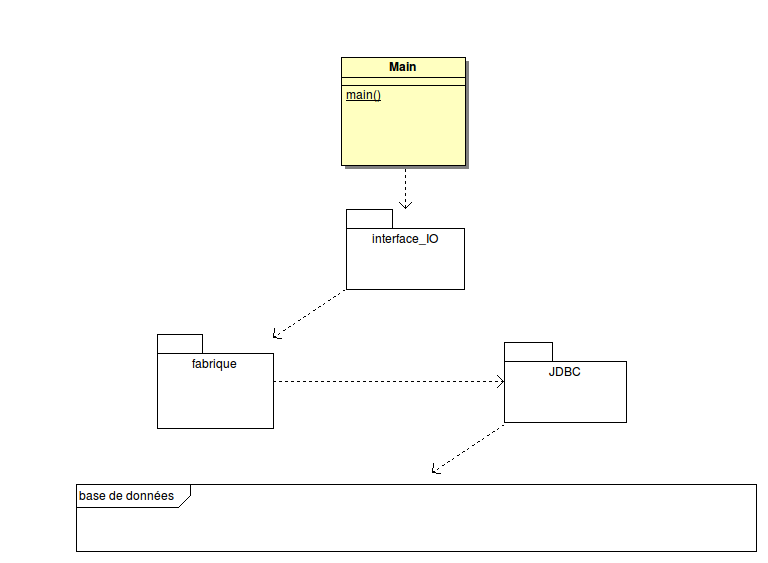
\includegraphics[width=14cm]{DiagClasseJavaPackage.png}
\end{center}
\mbox{}\hspace{0.4cm}Cette conception nous a amené à réaliser un paquetage par couche. Chaque paquetage ne pouvant faire appel que au premier paquetage en dessous de lui.\\
Lors de la conception nous n'avons eu l'impression que la couche \textit{application} n'était pas necessaire pour ce projet (Il s'est averé sur la fin, que cette couche aurait tout de même permit d'épurer les couches \textit{interface} et \textit{domaine} de partie algorithmique).\\
\mbox{}\hspace{0.4cm}Nous avons tout d'abord conçu la couche \textit{interface}, dont voici le diagramme de class.\\
\begin{center}
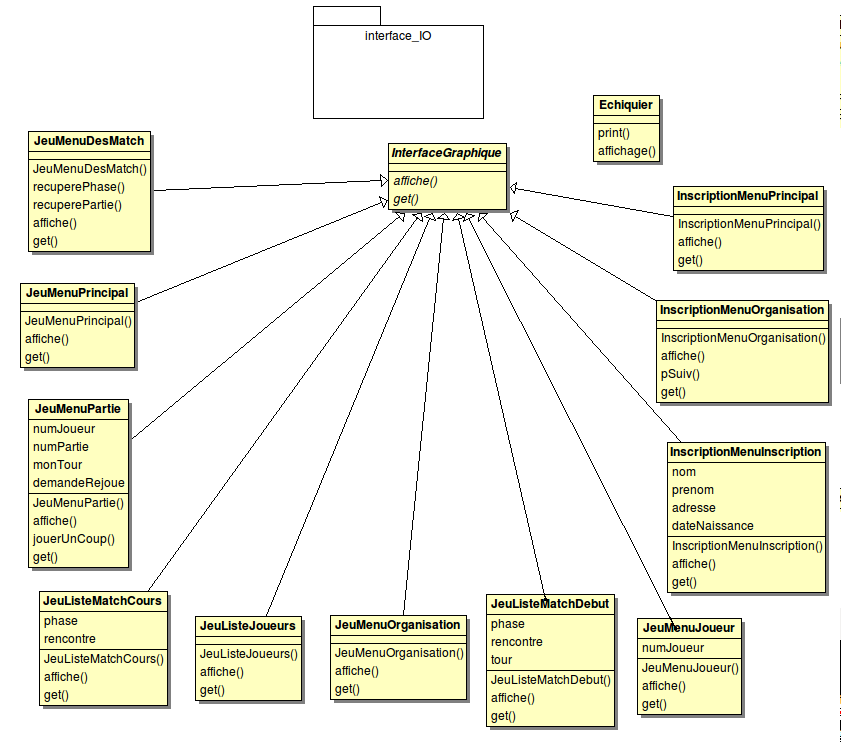
\includegraphics[width=18cm]{DiagClasseJavaInterface.png}
\end{center}
Dans cette couche se trouve dont une class abstrait \textit{interfaceGraphique} qui va nous permet de faire la liaison avec l'utilisateur (affichage, et recuperation des choix de l'utilisateur). Beaucoup de class sont étendus de la class abstrait, elles correspondent chacune a un \textit{Menu} différent. Nous avons aussi dans cette couche une class \textit{Echiquier} qui correspond a notre affichage de l'échiquier (cette class est utilisé à plusieurs reprises par des class \textit{Menu}).\\
Voici un diagramme qui represente les différents appels possibles des class entre elles dans la couche \textit{interface}\\
\begin{center}
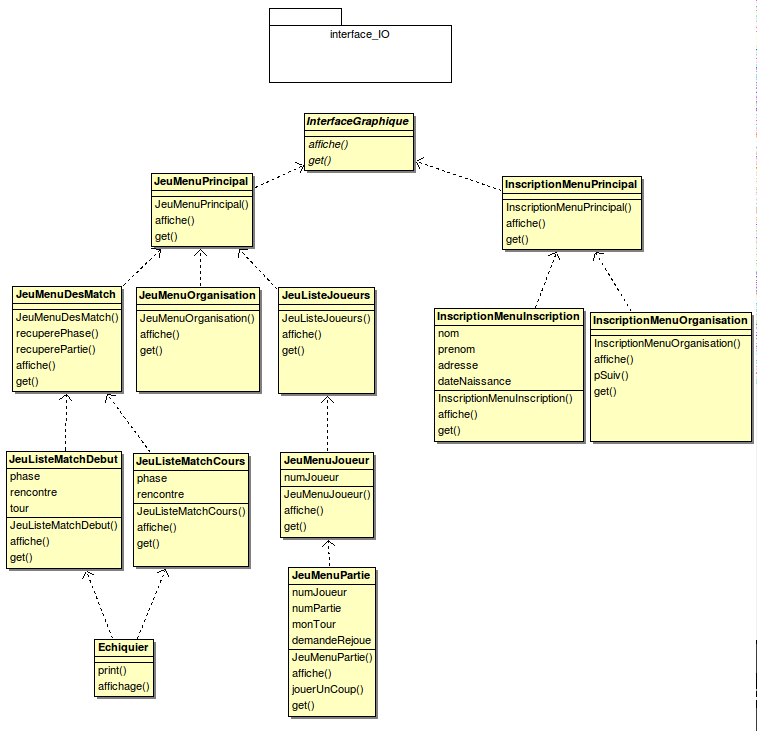
\includegraphics[width=18cm]{DiagLienJavaInterface.png}
\end{center}
\mbox{}\hspace{0.4cm}Nous avons aussi conçu la couche \textit{domaine} pour laquelle nous avons utilisé le patron \textit{interface}.\\
\begin{center}
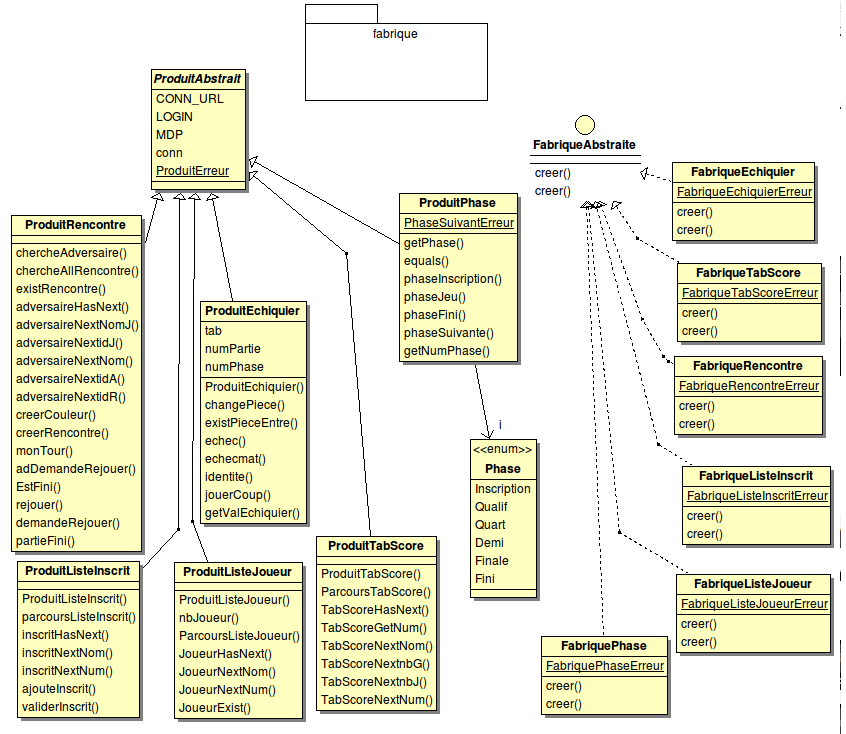
\includegraphics[width=18cm]{DiagClasseJavaFabrique.png}
\end{center}
Pour cette couche nous avons commencé par identifier un par un, les différents objets, informations qui seront necessaire à l'implementation de l'application. Nous avons ensuite créer un objet concret par élément identifié. De plus nous avons utlisés l'API \textit{jdbc} afin de faire les requetes sql.

\section{Implémentation de l'application}
\subsection{Paquetage \lstinline!interface\_IO!}
\begin{itemize}
\item \lstinline!Echiquier.java!: Permet l'affichage de l'échiquier.
\item \lstinline!InterfaceGraphique.java!: classe abstraite, de laquelle étendent toutes les classes ci-dessous.
\item \lstinline!InscriptionMenuPrincipal.java!: Menu principal lors de la phase d'inscription.
\item \lstinline!InscriptionMenuOrganisation.java!: Menu permettant à l'organisateur de valider les demandes d'inscription et de passer à la phase suivante.
\item \lstinline!InscriptionMenuInscription.java!: Menu permettant à un spectateur de s'incrire.
\item \lstinline!JeuMenuPrincipal.java!: Menu principal lors des phases de jeu.
\item \lstinline!JeuMenuOrganisation.java!: Menu permettant à l'organisateur de visualisé le tableau des scores de la phase en cours, et de passer à la phase suivante.
\item \lstinline!JeuMenuDesMatch.java!: Menu permettant à un spectateur de choisir une rencontre, et de choisir s'il veut la vivre en direct, ou reprendre depuis le début.
\item \lstinline!JeuListeMatchDebut.java!: Menu permettant à un spectateur de regarder une rencontre depuis le début.
\item \lstinline!JeuListeMatchCours.java!: Menu permettant à un spectateur de regarder une rencontre en direct.
\item \lstinline!JeuListeJoueurs.java!: Menu permettant à un spectateur de s'identifier en tant que joueur.
\item \lstinline!JeuMenuJoueur.java!: Menu permettant à un joueur de choisir une partie sur laquel jouer.
\item \lstinline!JeuMenuPartie.java!: Menu permettant à un joueur de jouer sur un coup, faire une demande pour rejouer la partie, ou bien abandonner.
\end{itemize}

\subsection{Paquetage \lstinline!fabrique!}
Pour chacun des éléments de la liste suivante, il existe une fabrique
et un produit.
\begin{itemize}
\item \lstinline!Abstrait!: Les connexions à la base de données sont
  factorisées dans ce produit abstrait.
\item \lstinline!Echiquier!: Permet la gestion de l'échiquier. 
Dans ce produit, plusieurs fonctions nécessitent d'être éclairées:
\begin{itemize}
\item \lstinline!boolean echec(int numJoueur)!:
Cette fonction renvoie \lstinline!TRUE! si le joueur
\lstinline!numJoueur! est en échec dans la partie considérée. Pour
évaluer l'échec, on regarde si il existe une pièce adverse capable de
prendre le roi. On vérifie ensuite systématiquement si le joueur est
échec et mat.
\item \lstinline!boolean echecmat(int numJoueur)!: 
Cette fonction renvoie \lstinline!TRUE! si le joueur
\lstinline!numJoueur! est en échec et mat dans la partie
considérée. La situation d'échec et mat n'est vérifiée que si une
situation d'échec a été détéctée au préalable. Pour évaluer l'échec et
mat, on bouge toutes les pièces du joueur \lstinline!numJoueur! afin
de savoir s'il existe un déplacement d'une pièce telle que le joueur
n'est plus en situation d'échec. Afin d'accélérer l'algorithme, le
premier mouvement vérifié est celui du roi.
\item \lstinline!boolean jouerCoup(int iprec, int jprec, int i, int j, int idJoueur)!:
Cette fonction permet de jouer effectivement un coup, en modifiant la
position de la pièce dans la base de données. Cette dernière vérifiera
la validité du coup en fonction de la pièce considérée. Cependant,
afin d'éviter des accès inutiles à la BD, on vérifie d'abord que
certaines conditions sont remplies: y a-t-il une pièce sur cette case?
Cette pièce est-elle à moi? Existe-t-il une pièce entre ma case et la
case destination? Si la pièce est un pion, a-t-il le droit de faire ce
déplacement?\\
Une fois ces vérifications effectuées, on peut soumettre le
déplacement à la BD, c'est à dire mettre à jour les coordonnées de la
pièce et créer le tour correspondant.\\
Enfin, si le coup effectuée met le joueur en situation d'échec, ce
coup n'est pas valide: on remet la BD et la structure de données en
état et on informe le joueur.
D'autre part, si une pièce se trouve sur la case destination, il faut
la supprimer de la BD.\\
\end{itemize}
\item \lstinline!ListeInscrit!: Ce module permet la gestion des inscriptions.
\item \lstinline!ListeJoueur!: Ce module permet la gestion des joueurs.
\item \lstinline!Phase!: Ce module permet la gestion des phases.
\item \lstinline!Rencontre!: Ce module permet la gestion des
  rencontres.
Les fonctions principales de ce module sont les suivantes:
\begin{itemize}
\item \lstinline!void chercheAllRencontre(int idPhase)!: Cette
  fonction stocke dans une liste toutes les rencontres possibles pour
  une phase.
\item \lstinline!void creerRencontre(int idPhase, int idRencontre, int
  idJoueur1, int idJoueur2)!:
Cette fonction crée dans la base de données la rencontre.
\item D'autres fonctions permettant de rejouer une rencontre sont
  également dans le produit de ce module: demander à rejouer une
  rencontre ou encore réinitialiser la rencontre.
\item
\end{itemize}
\item \lstinline!TabScore!:  Ce module permet de gérer un tableau des scores.
\end{itemize}


\chapter{Bilan}
\paragraph{}Durant toute la durée du projet, nous avons séparé notre groupe de quatre en deux groupes de deux. Romain et Thibault ont travaillé sur toute la partie de bases de données, et Valmon et Romaric sur toute la partie java de l'application. Une fois encore, même avec cette séparation nous avons continué de travailler ensemble et de demander des informations à l'autre groupe afin que notre application reste cohérante.
Une des difficultés rencontrées dans le projet est apparue très tôt. En effet lors de la conception, il nous avaient paru difficile de faire des diagrammes complets et exhaustifs. Et lorsqu'on nous avons commencé à coder l'application et la base de données, nous avons du modifier certains digrammes et faire de la "rétro-conception".
Puis après réflexion, cela nous a paru contre productif et étant contraire à l'essence même de la conception. Nous avons donc repris toute la conception depuis le début, avec plus de recul. Puis sans retoucher à la conception nous en avons découler le code de l'application et de la base de données. C'est aussi une leçon que nous essayerons de retenir pour nos futur projets, car nous avons perdus beaucoup de temps sur ce point.
\paragraph{}

\chapter*{Mode d'emploi}
L'interface graphique de notre application est entièrement
textuelle. La navigation dans l'application se fait par saisie des
numéros demandés.\\
Dans la phase d'inscription, on peut soit accéder au menu
d'inscription, soit au menu organisateur. \\
Dans la phase de jeu, on peut soit accéder au menu de visionnage de
jeu, soit au menu de jeu, soit au menu organisateur.\\ \\

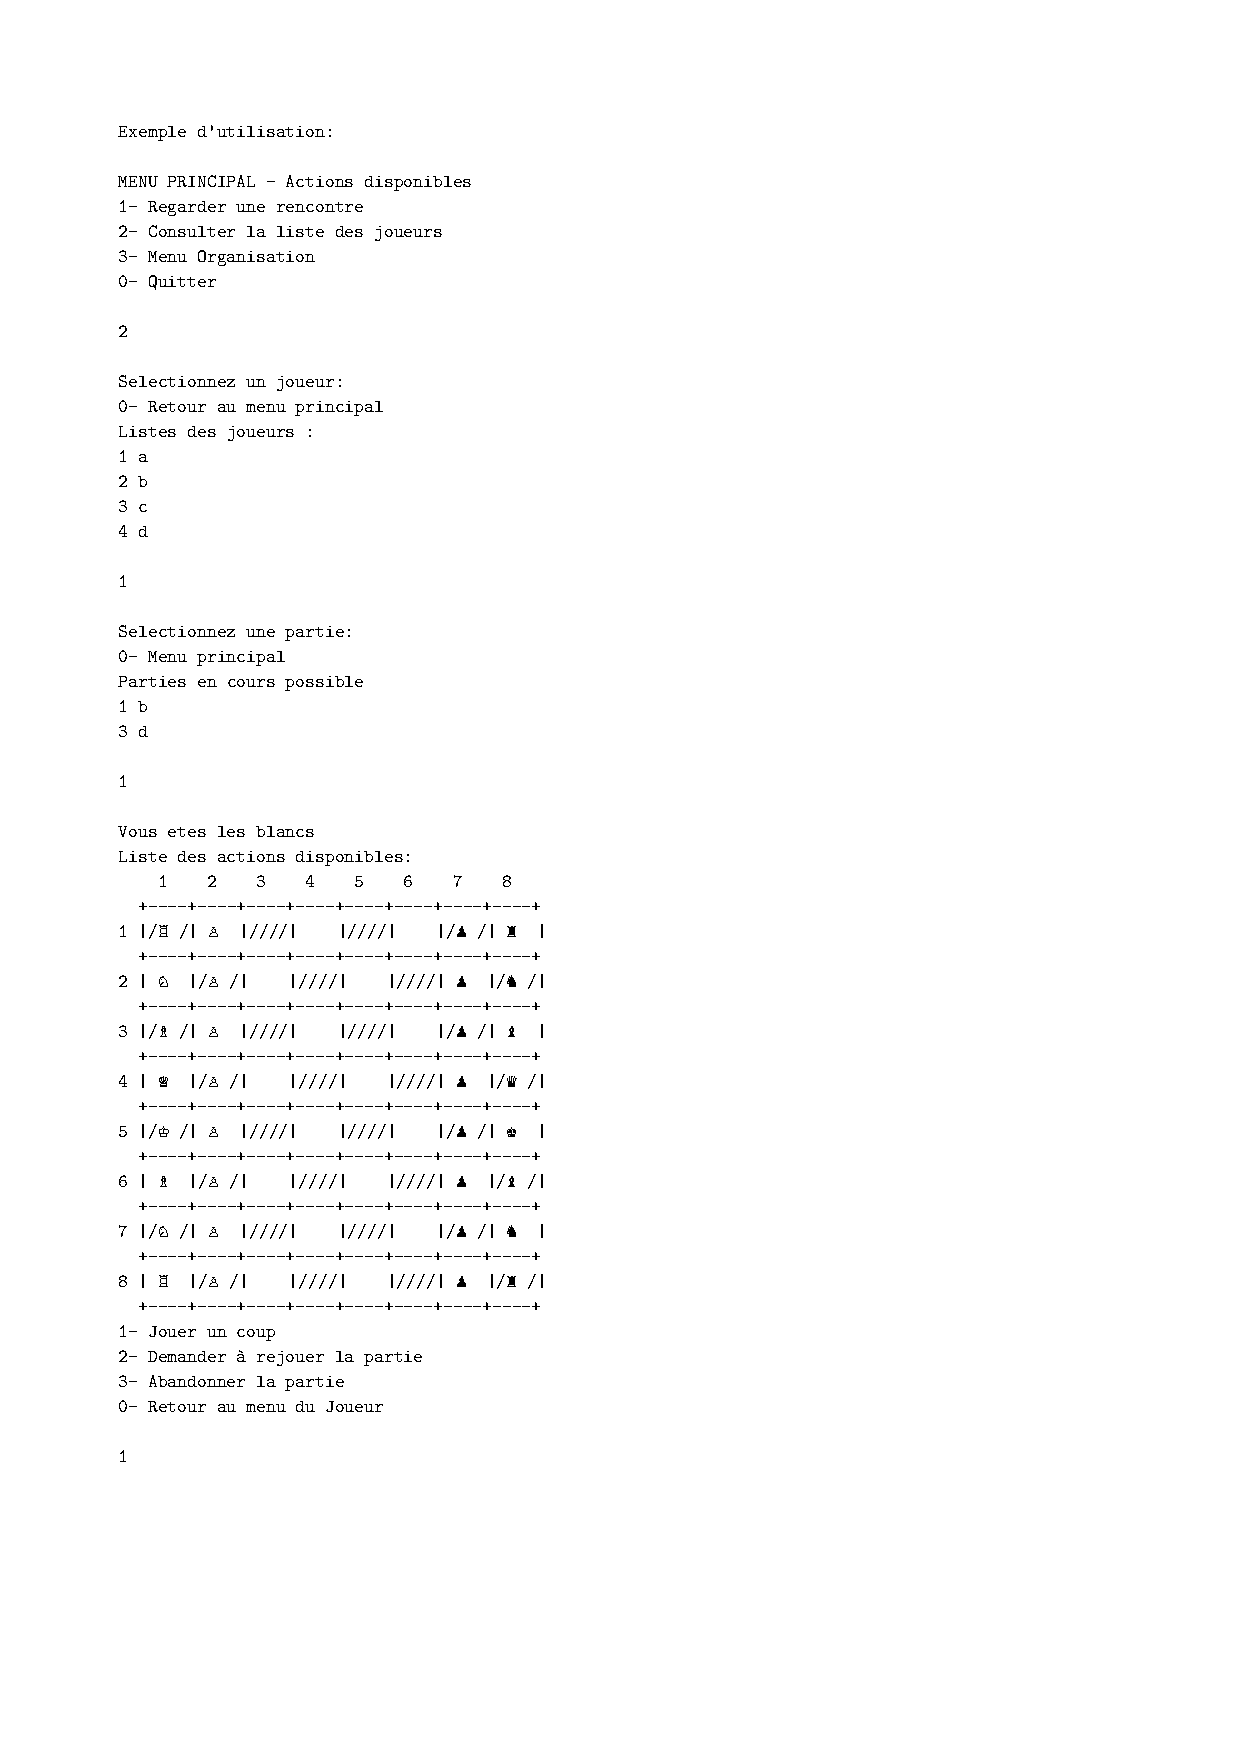
\includepdf[pages=1-2]{exUtilisation.pdf}

\end{document}
